
\chapter{Introduction \label{chap:01-Introduction}}

% First paragraph has no indentation.

\noindent Many researchers believe the computer has become the third
method to do research, in addition to theory and experimentation,
for both science and engineering. Although there is no complete agreement
on the position intended for scientific computing with respect to
the other two methods, it is undeniable that computational methods
are an essential tool in most disciplines, particularly in those related
to decision making.

Nowadays, decision making is present practically everywhere. As scientists,
engineers and managers have to make decisions in more complex and
competitive circumstances every day, decision making involves dealing
with rational and optimal approaches. According to Talbi~\cite{Talbi_Metaheuristics:2009},
decision making consists of the following steps:
\begin{itemize}
\item formulating the problem,
\item modeling the problem, 
\item solving the problem, and
\item implementing a solution for the problem.
\end{itemize}
Formulating a decision problem means making an initial statement about
it. Although this first formulation may be imprecise, the objectives
of the problem are outlined, together with the internal and external
factors that have some degree of influence over it. During the modeling
of the problem, an abstract mathematical model is built for it. Sometimes
this model is inspired by similar models in the literature, making
it possible to tackle the problem with well-studied methods. After
a model of the problem is available, one may start solving it. In
the context of this thesis, optimization means generating ``good''
solutions for the problem. It is important to note that the resulting
solutions are given for the abstract model, and not for the original
problem itself. Therefore, the performance of the obtained solution
is indicative when the model is an accurate one~\cite{Talbi_Metaheuristics:2009}.
In the last step, the obtained solution is practically tested by the
decision maker and implemented if it is an ``acceptable'' or ``good''
one. In case of ``bad'' or ``unacceptable'' solutions, the decision-making
process is repeated, possibly improving the model and/or the optimization
algorithm. The process, as described here, is depicted in Figure~\ref{fig:01-decision_making_process}.

\begin{figure}
\centering

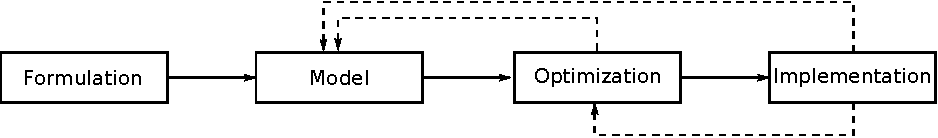
\includegraphics[width=0.75\textwidth]{01-introduction/img/decision_making_process}

\caption{A diagram of the classic decision-making process. Adapted from \cite{Talbi_Metaheuristics:2009}.\label{fig:01-decision_making_process}}
\end{figure}


\bigskip{}


Scientific computing, by means of computer-science methodology, enables
the study of problems that are too complex to be treated analytically,
or those that are very expensive or dangerous to be studied by direct
experimentation. Real-world problems are typically very complex systems
to be directly assessed by analytical models, and require a numerical
simulation for their study. Computer simulations provide a resource
to mimic the behavior of complex systems, by numerically evaluating
a model and gathering its data to estimate their true characteristics
\cite{law2007simulation}.

A model is a simplified representation of a studied problem, and one
of its purposes is to predict the effects of the variations within
the system. A good model is a balance between realism and simplicity.
The system simulation, on the other hand, is the operation of the
model. Its configuration can be changed, thus allowing multiple experimental
executions, something that might not be possible with the real system
it represents \cite{maria1997introduction}. However, it is important
to understand that the models used in scientific simulations and engineering
never offer a perfect representation of the system they resemble,
but only a subset of its composition and dynamics. For this reason,
experimentation and expert observation will always be essential as
reference points for understanding the studied phenomena. Consequently,
problems categorized as of large size and of considerable complexity
represent a challenge, because of the different involved disciplines
for their study and the degree of difficulty of their modeling. Cellular
radio networks in general, and those of the latest generations in
particular, fall under this categorization.


\section{Problem statement}

Radio networks represent one of the most fast-growing technology markets
since the introduction of the Global System for Mobile communications
(GSM\nomenclature[A]{GSM}{Global system for mobile communications})~\cite{3GPP_TR_50.099}.
As an implementation of the second generation of mobile networks (2G\nomenclature[A]{2G}{Second generation of mobile networks}),
GSM appeared more than twenty years ago. Its successor, the Universal
Mobile Telecommunications System (UMTS\nomenclature[A]{UMTS}{Universal mobile telecommunications system})~\cite{3GPP_TR_23.101}
marks an evolution from 2G, representing a milestone for the third
generation of mobile radio networks (3G\nomenclature[A]{3G}{Third generation of mobile networks}).
In recent years, the first commercial networks implementing the Long
Term Evolution (LTE\nomenclature[A]{LTE}{Long term evolution}), also
known as fourth generation (4G\nomenclature[A]{4G}{Fourth generation of mobile networks})
LTE, have also appeared~\cite{Gerstenberger-Introduction_to_LTE:2011}.
The always increasing demand for more bandwidth has been one of the
main forces behind the standardization and later implementation of
systems delivering higher-speed data services in order to improve
the user's experience.

This evolution, first from 2G to 3G and later from 3G to 4G, has introduced
not only the technology needed to increase data-transfer capacity
and voice quality, but also a greater complexity in terms of radio-network
planning, deployment, and configuration. This fact has attracted the
attention of the research community into areas such as the design
and optimization of radio-networks.

During the design phase of a radio network, a traditional or manual
approach comprises the software tool, i.e., the model in Figure~\ref{fig:01-decision_making_process},
that executes the analysis, and the human that makes the configuration
changes, i.e., the optimization in Figure~\ref{fig:01-decision_making_process}.
Therefore, a radio engineer manually adjusts the network parameters
and the software tool analyzes the given configuration. If the obtained
results are not acceptable, the analysis process has to be repeated
several times, until the goal is achieved and the changes are implemented,
i.e., the implementation in Figure~\ref{fig:01-decision_making_process}.
In the context of this thesis, this process is referred to as manual
radio-network optimization. 

Advances in the past few years have improved the manual optimization
process by introducing different problem-solving approaches that increase
the role of the computer during the optimization of radio networks,
consequently enlarging the scope of problems and instance sizes that
may be subject to optimization. Still, there are some important aspects
that restrict the automation level of these methods, not only in real-world
environments, but also when doing research in the area of radio networks:
\begin{itemize}
\item A selected optimization method is typically a compromise between solution
quality and computational-time complexity. The proposed state-of-the-art
approach for the evaluation of radio networks is the Monte-Carlo snapshot
analysis~\cite{Turke-Efficient_methods_for_WCDMA_radio_network_planning_and_optimization:2007,Wacker-Static_simulator_for_studying_WCDMA_radio_network_planning;1999}.
However, real-world environments, where radio-network design is carried
out, require the evaluation of networks with thousands of base stations
in a reasonable amount of time. Moreover, for applications involving
radio-network optimization, usually millions of evaluations are required
to find a good solution, in which case also snapshot simulations are
too time-consuming for practical use. Therefore, for such applications
and environments, methods with improved time efficiency are required.
\item A considerable number of publications in the field of radio-network
optimization, a few references of which are given for illustration
purposes~\cite{Amaldi-Radio_planning_and_coverage_optimization_of_3G_networks:2008,chen2008automated,Chen-Fast_algorithm_for_large_scale_UMTS_coverage_planning:2009,Antenna.azimuth.tilt:2009,Antenna.Configuration:2008,Siomina:Minimum.pilot.power.for.service.coverage},
base their simulations on platforms for which it is not possible to
reproduce the experiments, either because they have used proprietary
software or because the data is not available. This fact reduces the
possibilities for comparing different approaches among each other,
and significantly contrasts with other research areas, such as evolutionary
computing or numerical optimization, where several sets of open and
well-known benchmarks are available for the community to use. Consequently,
an open and unified framework should allow researchers to compare
different methods and results in a simplified and objective manner.
\item Available commercial tools for radio-network evaluation present several
drawbacks. In particular, regarding the size of networks that can
be considered and their computational-time complexity. Yet, even if
precise and fast methods were commercially available, they would lack
the level of flexibility required by the scientific community. Consequently,
an essential attribute of the framework is to be open source, so that
anyone can extend it to meet some specific requirements. In the long
term, this process should also extend the set of built-in functionality.
\item Particularly for path-loss predictions, estimated with empirical or
deterministic mathematical models, the inaccuracy of the input data
directly deteriorates the precision of the calculated results. Moreover,
since the physical properties that influence the propagation of radio
signals are not constant and every environment introduces its own
deviations, the calculated prediction may be considered as not more
than a rough approximation. Therefore, there is a need for a technique
that improves the accuracy of the state-of-the-art mathematical models
for radio propagations, despite the various sources of error noted
before.
\end{itemize}
This thesis introduces methods and tools to mitigate the above-mentioned
drawbacks from a radio-planning perspective.


\section{Hypotheses and approaches}

The work presented in this thesis is based on the following hypotheses
and their related approaches:
\begin{itemize}
\item Applying parallelization techniques should reduce the computational-time
requirement of the radio-propagation prediction, thus making it possible
to process larger, real-world radio networks.

\begin{itemize}
\item Unlike several examples in the literature of radio-network simulators,
which do not include support for parallel methods in order to reduce
the computational-time complexity, the unified framework includes
this feature in its basic structure. In this sense, parallel techniques
are used even when targeting a single computing host.
\end{itemize}
\item Using hardware, specialized for parallel execution (e.g., GPU), should
improve the execution time of parallel algorithms using threads or
message-passing mechanisms.

\begin{itemize}
\item From its arrival a few years ago, general GPU programming is continuously
gaining the attention of the research community and it is extending
to several areas of science. In particular, the combination of parallel-programming
techniques with GPU hardware should reduce the computational-time
requirement of the radio-propagation prediction even further.
\end{itemize}
\item Using the parallel framework for the objective-function evaluation
of different optimization problems should improve the quality of solutions
and enable tackling larger problem instances.

\begin{itemize}
\item On the one hand, a larger number of evaluations in the same amount
of time translates into a better exploration of the search space by
the optimization algorithm used. On the other hand, more complex or
exact models may be evaluated in the same amount of time, which implies
more accurate solutions.
\end{itemize}
\item Using the parallel framework to evaluate the objective function of
an automatic-optimization system should provide the means for solving
new, previously inaccessible optimization problems.

\begin{itemize}
\item The improved performance at the evaluation level opens new possibilities
for formally defining and tackling optimization problems that were
previously out-of-reach of state-of-the-art methods, either because
of their complexity or size.
\end{itemize}
\end{itemize}

\section{Scientific contributions}

The contributions of this thesis to the fields of telecommunications
and computer sciences include the following:
\begin{enumerate}
\item Design and development of a unified framework for radio-network planning
and optimization that supports computer clusters and GPUs.
\item Proposal of a new approach for parallel programming that enhances
the performance of a classic master-worker method.
\item Quality improvement of radio-propagation predictions by applying metaheuristic-optimization
techniques.
\item A new algorithm, based on autonomous agents, to tackle the service-coverage
problem in radio networks.
\item Identification and formalization of a new optimization problem in
radio networks.
\end{enumerate}

\section{Organization}

So far, a context has been provided for the following content of this
thesis. An introduction of the three research areas addressed by this
work, i.e., optimization, radio networks, and parallel methods, is
given in Chapters~\ref{chap:02-Optimization_models}, \ref{chap:02-Principles_of_mobile_radio_networks}
and~\ref{chap:02-Principles_of_GPU_programming}, respectively. They
provide an overview of the theoretical elements needed for a better
understanding of the rest of the thesis. Additionally, Chapter~\ref{chap:02-Optimization_of_radio_networks}
provides a short literature survey about the optimization of radio
networks. 

The unified framework for radio-network planning and optimization,
incorporating elements from the above-mentioned fields of study, is
presented in Chapter~\ref{chap:04-Framework-design-and-implementation}.

Chapters~\ref{chap:06-Experimental-evaluation-the-service-coverage-problem}
and~\ref{chap:07-Experimental-evaluation-the-SHO-alignment-problem}
demonstrate how the framework is applied to tackle two optimization
problems. In Chapter~\ref{chap:06-Experimental-evaluation-the-service-coverage-problem},
the problem of minimizing the total amount of pilot power subject
to a full coverage constraint is addressed with a novel approach.
Next, Chapter~\ref{chap:07-Experimental-evaluation-the-SHO-alignment-problem}
formally introduces a new optimization problem that deals with the
balancing of downlink and uplink soft-handover areas in UMTS networks.

The applicability and performance of the framework for radio-network
planning is validated in Chapters~\ref{chap:05-Framework_parameter_tuning}
and~\ref{chap:08-Real-world_network_planning}. Chapter~\ref{chap:05-Framework_parameter_tuning}
further extends the framework with automated-tuning capabilities that
enable its adaptation to different environments, thus improving the
accuracy of the radio-propagation predictions. In Chapter~\ref{chap:08-Real-world_network_planning},
the framework is tested in real network-planning conditions and compared
to a commercial, enterprise-level tool in terms of solution quality
and speed performance.

Finally, Chapter~\ref{chap:Conclusion} gives a short summary of
the thesis, outlines its main contributions and discusses further
work.


\section{Publications }

The work presented in this thesis is supported by a number of previous
publications. The initial work on the unified framework for radio-network
planning was published by Benedi\v{c}i\v{c} et al. in~\cite{Benedicic-A_GRASS_GIS_parallel_module_for_radio-propagation_predictions:2013}.
To address the challenges of the computational-time complexity during
optimization and its objective-function evaluations, Benedi\v{c}i\v{c}
et al. published the GPU extensions for the framework in~\cite{Benedicic-A_GPU_based_parallel_agent_optimization_approach:2013}.
The agent-based algorithm for solving the service-coverage problem
was initially published at the International multi-conference Information
Society~\cite{Benedicic_Pilot.power.optimization:2010}. This work
was further extended and later published in~\cite{Benedicic-A_GPU_based_parallel_agent_optimization_approach:2013}.
The primary ideas for the formal definition of the soft-handover balancing
problem were published at the World Congress of Computational Intelligence~\cite{Benedicic_Balancing_downlink_uplink_soft_handover_areas_in_UMTS_networks:2012}.
The results of the automated tuning capabilities of the framework
were published in~\cite{Benedicic-An_adaptable_parallel_simulation_framework_for_LTE_coverage_planning:2013}.

A comprehensive list of the author's publications is given in Appendix~A.
